% !TeX spellcheck = hu_HU
% !TeX encoding = UTF-8
% !TeX program = xelatex
% TODO Change language to en_GB (recommended) or en_US for English documents
\documentclass[11pt,a4paper,oneside]{report}             % Single-side
%\documentclass[11pt,a4paper,twoside,openright]{report}  % Duplex

% thanks to http://tex.stackexchange.com/a/47579/71109
\usepackage{ifxetex}
\usepackage{ifluatex}
\newif\ifxetexorluatex % a new conditional starts as false
\ifnum 0\ifxetex 1\fi\ifluatex 1\fi>0
   \xetexorluatextrue
\fi

\ifxetexorluatex
  \usepackage{fontspec}
\else
  \usepackage[T1]{fontenc}
  \usepackage[utf8]{inputenc}
  \usepackage[lighttt]{lmodern}
  \ttfamily\DeclareFontShape{T1}{lmtt}{m}{it}{<->sub*lmtt/m/sl}{}
\fi

\usepackage[english,magyar]{babel} % Alapértelmezés szerint utoljára definiált nyelv lesz aktív, de később külön beállítjuk az aktív nyelvet.

\usepackage{emptypage} % omit page number on empty pages

%\usepackage{cmap}
\usepackage{amsfonts,amsmath,amssymb} % Mathematical symbols.
%\usepackage[ruled,boxed,resetcount,linesnumbered]{algorithm2e} % For pseudocodes. % beware: this is not compatible with LuaLaTeX, see http://tex.stackexchange.com/questions/34814/lualatex-and-algorithm2e
\usepackage{booktabs} % For publication quality tables for LaTeX
\usepackage{graphicx}

%\usepackage{fancyhdr}
%\usepackage{lastpage}

\usepackage{anysize}
%\usepackage{sectsty}
\usepackage{setspace} % For setting line spacing

\usepackage[unicode]{hyperref} % For hyperlinks in the generated document.
\usepackage{xcolor}
\usepackage{listings} % For source code snippets.

\usepackage[amsmath,thmmarks]{ntheorem} % Theorem-like environments.

\usepackage[hang]{caption}

\usepackage{subfigure}

\singlespacing

\newcommand{\selecthungarian}{
	\selectlanguage{magyar}
	\setlength{\parindent}{2em}
	\setlength{\parskip}{0em}
	\frenchspacing
}

\newcommand{\selectenglish}{
	\selectlanguage{english}
	\setlength{\parindent}{0em}
	\setlength{\parskip}{0.5em}
	\nonfrenchspacing
	\renewcommand{\figureautorefname}{Figure}
	\renewcommand{\tableautorefname}{Table}
	\renewcommand{\partautorefname}{Part}
	\renewcommand{\chapterautorefname}{Chapter}
	\renewcommand{\sectionautorefname}{Section}
	\renewcommand{\subsectionautorefname}{Section}
	\renewcommand{\subsubsectionautorefname}{Section}
}

\usepackage[numbers]{natbib}
\usepackage{xspace}


%TODO Set the main variables
\newcommand{\vikszerzoVezeteknev}{Gáti}
\newcommand{\vikszerzoKeresztnev}{László Dávid}

\newcommand{\vikkonzulensAMegszolitas}{}
\newcommand{\vikkonzulensAVezeteknev}{Farkas}
\newcommand{\vikkonzulensAKeresztnev}{Rebeka}

\newcommand{\vikkonzulensBMegszolitas}{}
\newcommand{\vikkonzulensBVezeteknev}{}
\newcommand{\vikkonzulensBKeresztnev}{}

\newcommand{\vikkonzulensCMegszolitas}{}
\newcommand{\vikkonzulensCVezeteknev}{}
\newcommand{\vikkonzulensCKeresztnev}{}

\newcommand{\vikcim}{MagicDraw állapottérképek\linebreak formális verifikációja} % Cím
\newcommand{\viktanszek}{\bmemit} % Tanszék
\newcommand{\vikdoktipus}{\bsc} % Dokumentum típusa (\bsc vagy \msc)
\newcommand{\vikmunkatipusat}{szakdolgozatot} % a "hallgató nyilatkozat" részhez: szakdolgozatot vagy diplomatervet

\input{include/tdk-variables}
\newcommand{\szerzoMeta}{\vikszerzoVezeteknev{} \vikszerzoKeresztnev} % egy szerző esetén
%\newcommand{\szerzoMeta}{\vikszerzoVezeteknev{} \vikszerzoKeresztnev, \tdkszerzoB} % két szerző esetén

%TODO Language configuration -- choose one
% Beállítások magyar nyelvű dolgozathoz
%--------------------------------------------------------------------------------------
% Elnevezések
%--------------------------------------------------------------------------------------
\newcommand{\bme}{Budapesti Műszaki és Gazdaságtudományi Egyetem}
\newcommand{\vik}{Villamosmérnöki és Informatikai Kar}

\newcommand{\bmemit}{Méréstechnika és Információs Rendszerek Tanszék}

\newcommand{\keszitette}{Készítette}
\newcommand{\konzulens}{Konzulens}

\newcommand{\bsc}{Szakdolgozat}
\newcommand{\msc}{Diplomaterv}
\newcommand{\tdk}{TDK dolgozat}
\newcommand{\bsconlab}{BSc Önálló laboratórium}
\newcommand{\msconlabi}{MSc Önálló laboratórium 1.}
\newcommand{\msconlabii}{MSc Önálló laboratórium 2.}

\newcommand{\pelda}{Példa}
\newcommand{\definicio}{Definíció}
\newcommand{\tetel}{Tétel}

\newcommand{\bevezetes}{Bevezetés}
\newcommand{\koszonetnyilvanitas}{Köszönetnyilvánítás}
\newcommand{\fuggelek}{Függelék}
\newcommand{\uppaal}{UPPAAL}

% Opcionálisan átnevezhető címek
%\addto\captionsmagyar{%
%\renewcommand{\listfigurename}{Saját ábrajegyzék cím}
%\renewcommand{\listtablename}{Saját táblázatjegyzék cím}
%\renewcommand{\bibname}{Saját irodalomjegyzék név}
%}

\newcommand{\szerzo}{\vikszerzoVezeteknev{} \vikszerzoKeresztnev}
\newcommand{\vikkonzulensA}{\vikkonzulensAMegszolitas\vikkonzulensAVezeteknev{} \vikkonzulensAKeresztnev}
\newcommand{\vikkonzulensB}{\vikkonzulensBMegszolitas\vikkonzulensBVezeteknev{} \vikkonzulensBKeresztnev}
\newcommand{\vikkonzulensC}{\vikkonzulensCMegszolitas\vikkonzulensCVezeteknev{} \vikkonzulensCKeresztnev}

\newcommand{\selectthesislanguage}{\selecthungarian}

\bibliographystyle{huplain}

\def\lstlistingname{lista}

\newcommand{\appendixnumber}{6}  % a fofejezet-szamlalo az angol ABC 6. betuje (F) lesz

% Settings for English documents
%\input{include/thesis-en}

\input{include/preamble}

%--------------------------------------------------------------------------------------
% Table of contents and the main text
%--------------------------------------------------------------------------------------
\begin{document}

%TODO These define guidelines -- remove these
%~~~~~~~~~~~~~~~~~~~~~~~~~~~~~~~~~~~~~~~~~~~~~~~~~~~~~~~~~~~~~~~~~~~~~~~~~~~~~~~~~~~~~~
%\include{include/guideline}
%%--------------------------------------------------------------------------------------
% Feladatkiiras (a tanszeken atveheto, kinyomtatott valtozat)
%--------------------------------------------------------------------------------------



\selectthesislanguage

%TODO Titlepage -- choose one from below
%~~~~~~~~~~~~~~~~~~~~~~~~~~~~~~~~~~~~~~~~~~~~~~~~~~~~~~~~~~~~~~~~~~~~~~~~~~~~~~~~~~~~~~
\include{include/titlepage}		   % Szakdolgozat/Diplomaterv címlap
%\include{include/titlepage-tdk}	% TDK címlap
%\include{include/titlepage-otdk}   % OTDK címlap


% Table of Contents
%~~~~~~~~~~~~~~~~~~~~~~~~~~~~~~~~~~~~~~~~~~~~~~~~~~~~~~~~~~~~~~~~~~~~~~~~~~~~~~~~~~~~~~
\tableofcontents\vfill


% Declaration and Abstract
%~~~~~~~~~~~~~~~~~~~~~~~~~~~~~~~~~~~~~~~~~~~~~~~~~~~~~~~~~~~~~~~~~~~~~~~~~~~~~~~~~~~~~~
\include{include/declaration} %TODO Hallgatói nyilatkozat -- TDK és OTDK esetén törlendő!
\pagenumbering{roman}
\setcounter{page}{1}

\selecthungarian

%----------------------------------------------------------------------------
% Abstract in Hungarian
%----------------------------------------------------------------------------
\chapter*{Kivonat}\addcontentsline{toc}{chapter}{Kivonat}


Biztonságkritikus rendszerek tervezéséhez különösen fontos, hogy rendelkezésünkre álljanak olyan eszközök, melyek segítségével meg lehet vizsgálni, hogy a rendszer modellezett viselkedése valóban megfelel a rendszerrel szemben támasztott követelményeknek. A viselkedés modellezése magas szinten gyakran történik állapot alapú formalizmusokkal, mint például a UML állapottérképekkel. Ezek gyakran komponenseket definiálnak amik egymással kölcsönhatásban állnak, így szükségessé válik ezeknek a komponens együtteseknek a vizsgálata is. A tulajdonságok teljesüléséhez példákat kell szolgáltatni amik alátámasztják a tulajdonság teljesülését vagy adott esetben sérülését, hogy a mérnökök megtalálhassák és kijavíthassák a tervezési hibákat.

A MagicDraw egy UML és SysML modellező eszköz amely elterjedt az iparban. Ehhez az eszközhöz korábbi munkáim során készítettem egy beépülő modult, ami lehetővé teszi logikai formulák segítségével specifikált tulajdonságok teljesülésének ellenőrzését állapottérképeken. A mérnökök gyakran használnak hierarchikus, komponens alapú állapot modelleket rendszerek modellezésére, azonban a beépülő modul ezek együttes ellenőrzésére nem képes. A tulajdonságok teljesülésének vizsgálata olyan példák keresését jelenti, amik bizonyítják ennek teljesülését. Fontos, hogy a mérnökök ezekhez hozzáférjenek és elemezni tudják. A beépülő modul ezeket megjelenítésére nem képes.

Dolgozatomban bemutatom a beépülő modult és hogy milyen módon fejlesztettem azt tovább, hogy lehetőséget biztosítson komponenst alapú hierarchikus állapot modellek formális ellenőrzésére és az ellenőrzés során keletkező bizonyítékként szolgáló példák megjelenítésére. Az elkészítette eszköz működését egy példán keresztül bemutatom, majd mérések segítségével értékelem a gyakorlati megvalósítás hatékonyságát.


\vfill
\selectenglish


%----------------------------------------------------------------------------
% Abstract in English
%----------------------------------------------------------------------------
\chapter*{Abstract}\addcontentsline{toc}{chapter}{Abstract}

Safety critical systems raise the need for various tools that can verify their design by checking if modeled behaviors satisfy their specified requirements.

Modeling behaviors on a high level often relies on state-based formalisms such as UML statecharts. These often serve as definitions for components that influence each other’s behavior through various types of communication. This makes it necessary that the tools support this kind of modeling and allow model checking on such component-based systems. The existence of required system properties must be proven by examples that either prove or disprove the existence of these specified properties. Engineers then can use these examples to find and correct errors in the model.

MagicDraw is a modeling tool for UML and SysML and it is a widely used tool amongst system engineers. In the course of my previous works, I have made a plugin for this modeling tool which enables the check of properties defined as logical formulas on statecharts. However, it cannot perform checks on models that follow the commonly used component-based approach. The existence of properties is proven by finding examples as proof of their existence. It is important that engineers can view and analyze these examples which the tool does not allow just yet.

In my thesis I introduce the tool that I have made previously and the feature improvements that allow the checking of component-based systems and the display of examples produced during the checking process. I present my solutions on a small-scale example then I perform some measurements to evaluate the performance of the used solutions.


\vfill
\cleardoublepage

\selectthesislanguage

\newcounter{romanPage}
\setcounter{romanPage}{\value{page}}
\stepcounter{romanPage}    %TODO Összefoglaló -- TDK és OTDK esetén nem kötelező


% The main part of the thesis
%~~~~~~~~~~~~~~~~~~~~~~~~~~~~~~~~~~~~~~~~~~~~~~~~~~~~~~~~~~~~~~~~~~~~~~~~~~~~~~~~~~~~~~
\pagenumbering{arabic}

%TODO import your own content
%\pagenumbering{roman}
\setcounter{page}{1}

\selecthungarian

%----------------------------------------------------------------------------
% Abstract in Hungarian
%----------------------------------------------------------------------------
\chapter*{Kivonat}\addcontentsline{toc}{chapter}{Kivonat}


Biztonságkritikus rendszerek tervezéséhez különösen fontos, hogy rendelkezésünkre álljanak olyan eszközök, melyek segítségével meg lehet vizsgálni, hogy a rendszer modellezett viselkedése valóban megfelel a rendszerrel szemben támasztott követelményeknek. A viselkedés modellezése magas szinten gyakran történik állapot alapú formalizmusokkal, mint például a UML állapottérképekkel. Ezek gyakran komponenseket definiálnak amik egymással kölcsönhatásban állnak, így szükségessé válik ezeknek a komponens együtteseknek a vizsgálata is. A tulajdonságok teljesüléséhez példákat kell szolgáltatni amik alátámasztják a tulajdonság teljesülését vagy adott esetben sérülését, hogy a mérnökök megtalálhassák és kijavíthassák a tervezési hibákat.

A MagicDraw egy UML és SysML modellező eszköz amely elterjedt az iparban. Ehhez az eszközhöz korábbi munkáim során készítettem egy beépülő modult, ami lehetővé teszi logikai formulák segítségével specifikált tulajdonságok teljesülésének ellenőrzését állapottérképeken. A mérnökök gyakran használnak hierarchikus, komponens alapú állapot modelleket rendszerek modellezésére, azonban a beépülő modul ezek együttes ellenőrzésére nem képes. A tulajdonságok teljesülésének vizsgálata olyan példák keresését jelenti, amik bizonyítják ennek teljesülését. Fontos, hogy a mérnökök ezekhez hozzáférjenek és elemezni tudják. A beépülő modul ezeket megjelenítésére nem képes.

Dolgozatomban bemutatom a beépülő modult és hogy milyen módon fejlesztettem azt tovább, hogy lehetőséget biztosítson komponenst alapú hierarchikus állapot modellek formális ellenőrzésére és az ellenőrzés során keletkező bizonyítékként szolgáló példák megjelenítésére. Az elkészítette eszköz működését egy példán keresztül bemutatom, majd mérések segítségével értékelem a gyakorlati megvalósítás hatékonyságát.


\vfill
\selectenglish


%----------------------------------------------------------------------------
% Abstract in English
%----------------------------------------------------------------------------
\chapter*{Abstract}\addcontentsline{toc}{chapter}{Abstract}

Safety critical systems raise the need for various tools that can verify their design by checking if modeled behaviors satisfy their specified requirements.

Modeling behaviors on a high level often relies on state-based formalisms such as UML statecharts. These often serve as definitions for components that influence each other’s behavior through various types of communication. This makes it necessary that the tools support this kind of modeling and allow model checking on such component-based systems. The existence of required system properties must be proven by examples that either prove or disprove the existence of these specified properties. Engineers then can use these examples to find and correct errors in the model.

MagicDraw is a modeling tool for UML and SysML and it is a widely used tool amongst system engineers. In the course of my previous works, I have made a plugin for this modeling tool which enables the check of properties defined as logical formulas on statecharts. However, it cannot perform checks on models that follow the commonly used component-based approach. The existence of properties is proven by finding examples as proof of their existence. It is important that engineers can view and analyze these examples which the tool does not allow just yet.

In my thesis I introduce the tool that I have made previously and the feature improvements that allow the checking of component-based systems and the display of examples produced during the checking process. I present my solutions on a small-scale example then I perform some measurements to evaluate the performance of the used solutions.


\vfill
\cleardoublepage

\selectthesislanguage

\newcounter{romanPage}
\setcounter{romanPage}{\value{page}}
\stepcounter{romanPage}
%----------------------------------------------------------------------------
\chapter{\bevezetes}
%----------------------------------------------------------------------------

A IT technológiák térnyerésével egyre több és komplexebb rendszer készül, melyeknek sokszor valós időben kell működni. Mivel ilyen rendszerek jellemzően valamilyen biztonság kritikus környezetben működnek, elengedhetetlené válik ezek gondos megtervezése és átfogó vizsgálata különösen a helyes működés tekintetében.

A tervezés és ellenőrzés költséges, időigényes folyamat, ezért szükség van olyan eszközökre amelyek megkönnyítik vagy akár teljesen automatizálnak egyes folyamatokat. A tervezés során általában valamilyen modellvezért technikát alkalmaznak, melynek középpontjában a modellek állnak. A tervezés során elkészített tervek nagyon sok értékes információt tartalmaznak, melyeket újra fel tudunk használni és származtatni ezekből kódot, dokumentációt, vagy akár más modelleket, ezáltal időt és erőforrásokat megtakarítva. Ráadásul mivel ezeket automatikusan gépek végzik, minimalizálódnak az emberi hibák például a programkódban, ahhoz képest mintha ezeket kézzel végeznénk el.

Terveinket már érdemes a tervezés korai fázisaiban ellenőrizni, hiszen az itt vétett hibák akár kritikusak lehetnek a későbbiekben. Az ellenőrzésekhez szintén fel tudjuk használni a modelljeinket és szimulálni tudjuk a rendszert, vagy képesek vagyunk magát a modellt is vizsgálni formális módszerek segítségével.

A MagicDraw egy mára de-facto ipari standarddá vált szoftver, és rendszer architektúra modellező eszköz ami fejlett grafikus interfészt nyújt a felhasználók számára. Modelleket elsősorban egy általános célú modellezési nyelvvel UML-el lehet készíteni, azonban UML profilok segítségével akár saját szakterület specifikus nyelvek használatára is lehetőségünk nyílik. Ilyen formában a MagicDraw lehetővé teszi modellek létrahozását SysML nyelven is amihez a profilt maga biztosítja. A dolgozat a továbbiakban SysML modellekkel foglalkozik.

Ugyan a MagicDraw számos fontos és hasznos funkcióval rendelkezik, még mindig megvan az igény újabbakra főleg Verifikáció/Validáció tekintetében. A MagicDrawToGamma nevű MagicDrawhoz készült plugin SysML állapottérképek formális verifikálásához nyújt megoldást, melyhez a Gamma Statechart Composition Frameworköt és az UPPAAL nevű eszközöket használja fel.

Az eszköz ugyan \emph{Proof of Concept} jelleggel már képes a verifikációt elvégezni, azonban, hogy akár szélesebb körben is használható eszközzé válhasson még sok tekintetben fejlesztésre szorul. Jelen dolgozat célja bemutatni azokat a fejlesztéseket amiket a mesterképzés során végeztem az eszközön és visszatekintve kiértékelni azokat a mérnöki megoldásokat melyeket a fejlesztés során hoztam.

A dolgozat felépítése a következő: a második fejezetben ismertetem azokat az ismereteket amelyek a dolgozat során felvetülő problémák illetve az ezekre adott megoldások megértéséhez szükségesek. A harmadik fejezetben ismertetem a projekt céljait és az ezekhez vezető utat, alkalmazott megoldásokat, illetve bemutatom a beépülő modul működését. A negyedik fejezetben pedig értékelem az alkalmazott megoldások hatékonyságát és az elkészített plugint.
\chapter{Bevezetés}
\chapter{Háttérismeretek}
\section{Modellek}

Modelleket az élet számos területén alkalmazunk, ez lehetővé teszi az előtt vizsgálni a megvalósítandó rendszert, hogy azt ténylegesen létre kellene hozni. A vizsgálatoknak számos módja és célja lehetséges. A látvány tervező bemutat egy látványtervet és a megfelelő stakeholderek ezt értékelik, vagy egy rendszerről komplex matematikai módszerekkel kell eldönteni, hogy stabil-e. A modellek leírása sokféle módon történhet, de célszerű egy olyan standardizált jelölési rendszert alkalmazni, hogy a többi szakember is értelmezni, vizsgálni tudja a modellt.

A jelölési rendszer vagy modellezési formalizmus lehet egy szöveges leírás is, például egy programkód, de sokszor célszerű vizuális megoldást használni, szimbólumokat tartalmazó diagramokat alkalmazni. Ezek sok esetben kifejezőbbek, lényegre törőbbek, és elsősorban könnyebben értelmezhetőek mint a szöveges leírások.

\section{Statechart formalizmus}

Az állapottérkép egy diagram ami irányított gráfot tartalmaz, ahol a csomópontok állapotokat, az élek állapotátmeneteket definiálnak. Az állapotok és átmenetek egy állapot alapú viselkedést írnak le amit állapotgépnek nevezünk. Az állapotátmenetek állapotok közötti lehetséges átjárásokat definiálnak és általában feltételhez kötöttek, ami jellemzően valamilyen esemény bekövetkezése vagy logikai feltétel teljesülése. A feltételek teljesülésekor az állapotváltás bekövetkezik, ezt szokás \emph{tüzelésnek} is hívni. Az állapotgép legfőbb jellemzője, hogy adott időpillanatban melyik állapotok aktívak, állapotváltások aktív állapotból történnek, ilyenkor az állapot inaktívvá válik a cél pedig aktívvá (hurok él is lehetséges).

A viselkedés indulásakor az első aktív állapotot kezdő állapotnak hívják, ez egy különleges ún. pszeudoállapot, ami az állapotgép belépési pontja és általában azonnal átléptetésre kerül egy másik állapotba.

\subsection{Állapottérképek UML 2-ben}
Előzőekben az állapot alapú modellezés kvázi alapjai kerültek bemutatásra. A következőkben az állapottérképek egy konkrét specifikációja kerül bemutatásra az UML 2 szerint.

\begin{itemize}
	%--------------
	% Állapot
	%--------------
	\item \emph{Állapot (State)}: az állapottérképek csomópontjai, a rendszer működésének egyfajta jól megkülönböztethető fázisai, amelyek valamilyen esemény bekövetkezésére várnak. Az állapotok rendelkeznek:
	\begin{itemize}
		\item név: az állapot neve
		\item be/kilépési akció: be és kilépés során végrehajtandó cselekvés.
	\end{itemize}
	
	%-----------------
	% Kezdő állapot
	%-----------------
	\item \emph{Kezdő állapot (Initial State)}: pszeudoállapot, régiónként egy szerepelhet belőle és a régió belépési pontjaként szolgál.
	%-----------------
	% Végső állapot
	%-----------------
	\item \emph{Végállapot (Final State)}\footnote{UML 2-ben a végső állapotot nem pszeudoállapotként hanem állapotként van definiálva https://www.omg.org/spec/UML/2.0} (final state): A végső állapot, a régió terminálasi pontja, ha egy állapotgép összes régiója egy végső állapotba ért akkor az állapotgép is terminál.
	%----------------
	% Termináló állapot
	%----------------
	\item \emph{Termináló állapot (Terminal State)}: pszeudoállapot, ami az egész állapotgépet azonnal terminálja, ezt hibák lekezelésére lehet például alkalmazni.
	%--------------
	% Állapot átmenet
	%--------------
	\item \emph{Állapot átmenet (Transition)}: az állapottérképek élei, a lehetséges állapotváltozásokat definiálják. Az állapotátmenetek rendelkeznek:
		\begin{itemize}
			\item Triggerekkel
			\item Őrfeltételekkel
		\end{itemize}
	%---------------
	% Trigger
	%---------------
	\item \emph{Trigger}: Állapot váltást kiváltó esemény amely lehet:
	\begin{itemize}
		\item Változás esemény (Change Event): valamilyen értéknek a megváltozása.
		\item Üzenet esemény (Message Event): valamilyen üzenet típusú objektumnak az érkezése, amit ebben a kontextusban kérésnek felel meg. Az ilyen típusú kommunikáció kétféle eseménytől függ, az üzenet elküldésétől és annak küldőjétől és az üzenet fogadásától és fogadójától. A kérés lehet egy metódus hívás, egy jelnek (\emph{Signal}) a fogadása.
		\item Időzítés esemény (Time Event): idő változásához kötött esemény.
	\end{itemize}

\end{itemize}
Fontos megjegyezni, hogy a dolgozat nem tér ki részletesen az események kiváltásának kérdésére, valamint az események küldésénél és fogadásánál szerepet játszó portokra, és interfészekre, ezen elemek a dolgozat szempontjából irrelevánsnak tekinthetők.
\begin{itemize}
	%----------------
	% Guard
	%----------------
	\item\label{sec:guard} \emph{Őrfeltétel (Guard)}: tágabb értelemben egy logikai kifejezés, melynek teljesülnie kell, hogy az adott állapotátmenet bekövetkezhessen. UML-ben ezek megszoríráskén \emph{(Constraint)} vannak értelmezve, ebben az értelemben a megszorításnak való megfelelés az állapotváltás feltétele.
	%----------------
	%Action
	%----------------
	\item \emph{Akció}: Különböző események bekövetkezésekor, mint állapotváltások, belépés állapotokba, kilépés állapotokból, vagy maga az állapotban maradás, lehetőségünk van viselkedéseket végrehajtani. UML szerint ezek lehetnek: Activityk, Állapotgépek, Interakció\footnote{Interakció modell elemek között, leírásához a jellegétől függően többféle diagram használható(Szekvencia, Kommunikációs, Időzítés).} OpaqueBehavior\footnote{ szöveges, UML-től eltérő nyelvvel specifikált viselkedés.}
	
	%-----------------
	% Ábra: állapot-atmenet-trigger-guard-action
	%----------------
	\begin{figure}[!ht]
		\centering
		
\includegraphics[keepaspectratio]{figures/statechart_elements/states.png}
		\caption{Állapotok és köztük definiált állapotátmenet, triggerrel, őrfeltétellel és actionnel}
	\end{figure}
	%----------------
	% Összetett állapot
	%----------------
\end{itemize}
Gyakran előfordul, hogy általánosabb állapotot célszerű felbontani részállapotokra. Az egyszerű állapottérképek elemeivel, ez a fajta hierarchikus viszony az állapotok között nehezen ábrázolható, ezért célszerű további elemek használata.
\begin{itemize}	
	%------------------
	% Régió
	%------------------
	\item \emph{Régió}: állapotokat tartalmazó egység, az állapottérkép mindig tartalmaz egy régiót amibe az állapotok definiálhatók. Régiók létezhetnek egymással párhuzamosan ilyenkor a végrehajtásuk párhuzamosan történik.
	%------------------
	% Öszetett állapot
	%-------------------
	\item \emph{Összetett állapot(Composite State)}: ha az állapotnak vannak további belső állapotai is, ha az állapot aktív akkor legalább egy belső is aktív, ha az állapotgép egy állapotváltás hatására kilép a kompozit állapotból akkor a belső állapotokból is kilép.
	%---------------
	% History state
	%--------------
	\item \emph{History State}: olyan pszeudo állapot, amely egy régióban megjegyzi az utolsó aktív állapotot, kilépéskor, ha a régióba visszalépünk a history state visszaállítja a megjegyzett állapotot. Amennyiben nincs előző állapot az ő belőle húzott állapotátmenet cél állapota lesz aktív. Két féle History Statet különböztetünk meg Shallow és Deep Historyt. Előbbi csak adott régión belül jegyzi meg az állapotot míg utóbbi a tartalmazott régiók állapotait is megjegyzi és visszaállítja.
	
\end{itemize}
Rendszerünket egy időpillanatban több egymástól független állapot is jellemezheti. Ezt a viselkedést párhozamos régiók alkalmazásával lehet leírni.
\begin{itemize}
	%------------------
	% Ortogonális állapot
	%------------------
	\item \emph{Ortogonális állapot (Orthogonal State)}: olyan összetett állapot ami két vagy több régiót tartalmaz.
	%---------
	% Fork
	%---------
	\item \emph{Fork}: pszeudoállapot, ami egy beérkező átmenetet szétbont több átmenetre, amiknek a cél állapotuk ortogonális régiókban találhatók. A kimenő átmeneteken nem lehet se trigger, sem pedig őrfeltétel.
	%---------
	% Join
	%---------
	\item \emph{Join}: pszeudoállapot, ami több beérkező átmenetet kapcsol össze eggyé. Az átmenetek ortogonális régiókból kell, hogy induljanak és nem lehet rajtuk trigger vagy őrfeltétel. A join szinkronizációs funkcionalitással bír: addig nem lehet tovább lépni belőle amíg minden beérkező átmenet végre nem hajtódott.
	
	\emph{Fork/Join} alkalmazásával ki tudjuk kényszeríteni, hogy részrendszereink elérjenek egy adott állapotot, mielőtt a végrehajtás folytatódhatna. Szintaktikájuk \aref{fig:forkjoin} ábrán látható. 
	
	%------------
	% Ábra: fork - join
	%-----------
	\begin{figure}[!ht]
		\centering
		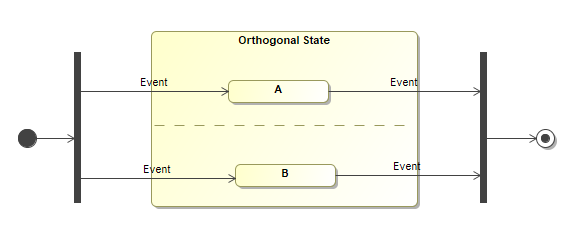
\includegraphics[keepaspectratio, width=100mm]{figures/statechart_elements/forkjoin.png}
		\caption{Példa: fork-join}
		\label{fig:forkjoin}
	\end{figure}
	
\end{itemize}
Rendszereink leírásakor előfordulhatnak ismétlődő részek, amiket célszerű egyszer leírni és újra felhasználni.
\begin{itemize}
	%-------------------
	% Submachine state
	%-----------------
	\item \emph{Submachine state}: Egy olyan állapot, ami egy állapottérképre hivatkozik, ez lehetővé teszi, hogy egy állapottérkép többszöri felhasználását, akár más-más kontextusban
	%---------------
	% Belépési pont
	%---------------
	\item \emph{Belépési pont(Entry Point)}: egy pszeudoállapot, ami egy állapotgép vagy egy kompozit állapot belépési pontját reprezentálja, célja egységbe zárni az állapotot vagy az állapotgépet. Továbbá léteznie kell egy állapotátmenetnek közte és egy az állapot vagy állapottérkép fő régiója között.
	%--------------
	% Kilépési pont
	%---------------
	\item \emph{Kilépési pont(Exit point)}: mint a belépési pont, de ez kilépési pontot reprezentál
	%---------------
	% kapcsolódási pont
	%---------------
	\item \emph{Kapcsolódási pont referencia(Connection Point Reference)}: \emph{Submachine Stateben} definiált be és kilépési pontokra tudunk vele hivatkozni, ez lehetővé teszi, hogy a \emph{Submachine Stateben} leírt belső állapotokhoz is felvehessünk állapotátmeneteket.
	
\end{itemize}
Egy állapottérképen a belépési és kilépési ponttal élek lehetséges kezdő illetve végpontjait tudjuk definiálni. Újrafelhasználásnál a behivatkozott állapottérképen ezekre referálhatunk Kapcsolódási Pont Referenciákkal. Az ezekbe húzott állapotátmenetek úgy tekintendők mintha kezdő vagy végpontjuk az az állapot lenne amihez a belépési vagy kilépési rendelve van. A \emph{Submachine State} szintaktikáját és használatát  \aref{fig:SubmachineState} ábra szemlélteti.
%-----------------
% Ábra Submachine state usage
%-----------------
\begin{figure}[!ht]
	\centering
	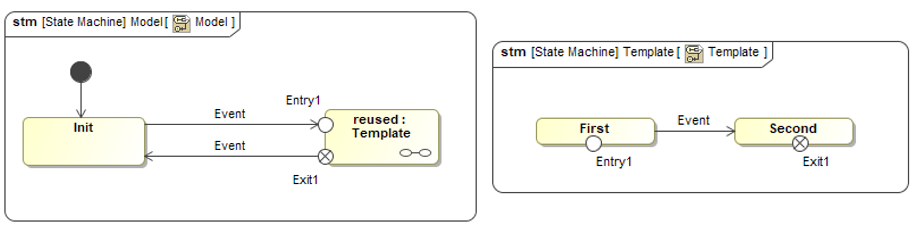
\includegraphics[keepaspectratio, width=150mm]{figures/statechart_elements/SubmachineState.png}
	\caption{Állapottérkép újrafelhasználása Submachine State segítségével}
	\label{fig:SubmachineState}
\end{figure}
\linebreak Logikailag állapotátmenetek is összetartozhatnak, ezért célszerű bizonyos esetekben egyesíteni, vagy szétbontani őket több alternatív átmenetre.
\begin{itemize}
	%-------------
	% Csomópont
	%-------------
	\item \emph{Csomópont (Junction)}: pszeudoállapot, több állapotátmenet összekapcsolása és egyként kezelése, például ha a cél állapotuk ugyan az és logikailag összetartoznak vagy egy beérkező átmenet szétbontása több átmenetre. Ilyenkor lehetőség van őrfeltételt rakni az átmenetekre, ezeknek a kiértékelése viszont még azelőtt történik, hogy bármelyik átmenet végrehajtásra kerülne, ezért egy ilyen ágat szokás statikus feltételes ágnak nevezni.
	%------------
	% Elágazás
	%-----------
	\item \emph{Döntés (Choice)}: hasonló mint a csomópont, viszont az őrfeltételek az elágazásba való belépéskor értékelődnek ki dinamikusan. Ezt jellemzően alternatív útvonalak megadására használjuk, hasonló mint a programozási nyelvekben \emph{"if than else"} elágazás. Fontos megjegyezni, hogy az elágazás és a csomópont esetében is lehetséges, hogy több átmenet is tüzelhetne, ilyenkor az érvényre jutó átmenet kiválasztása nem determinisztikus módon történik ezért elkerülendő, például \emph{else} őrfeltétel alkalmazásával.
	
	%-----------------
	% Ábra
	%-----------------
	%\begin{figure}[!ht]
	%	\centering
	%	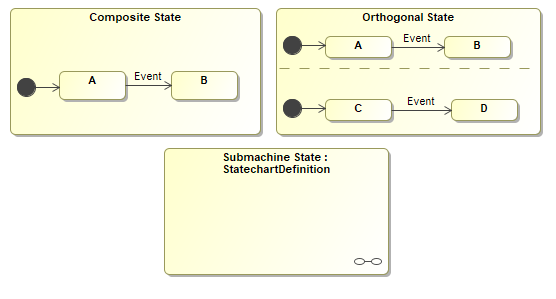
\includegraphics[keepaspectratio]{figures/statechart_elements/composit.png}
	%	\caption{Összetett állapot (balra), ortogonális állapot (jobbra) és submachine state (alul)}
	%\end{figure}
	
	
	
\end{itemize}

\section{MagicDraw}
A MagicDraw a No Magic \cite{NoMag} nevű cég által fejlesztett modellező eszköz, amivel a modellek előállításán kívül lehetőségünk van ezeket szimulálni, validálni, vagy akár kóddá alakítani. Az eszköz első sorban UML modelleket lehet készíteni, de plug-innal lehetőségünk van SysML \cite{SysML} modelleket is létrehozni.

A SysML egy általános-célú modellezési nyelv ami az UML egy részének kiragadásával és annak kibővítésével keletkezett. SysMLel struktúrát és viselkedést lehet leírni magas szinten. Alapeleme a Blokk, ami UML-ben a Classnak felel meg. A Blokk egy absztrakt egység ami bárminek megfeleltethető, így a modellezendő rendszer is általában egy Blokként jelenik meg. A Blokkok definícióját és tartalmazási hierarchiáját Block Definition Diagramokkal írhatjuk le. Egy másik megemlítendő diagramfajta az Internal Block Diagram, amivel a Blokkok és portjaik között tudunk kapcsolatokat definiálni.

Viselkedést Állapottérképekkel és Activity Diagrammokkal szokás leírni SysMLben. Utóbbival munka- és adatfolyamokat, ahol a folyamat lépései activityk és actionök. Állapottérképekkel reaktív rendszereket szokás leírni, a rendszer eseményekre reagál, ezek határozzák meg a viselkedését, szemben az Activity Diagrammokkal, amivel adott bemenetből valamilyen kimenet előállításának folyamatát írjuk le.

\subsection{Állapottérképek SysMLben}
Az állapottérképeket SysML modellek részeiként, más modell elemekhez vannak viselkedésként hozzárendelve, a triggereket aktiváló események a modell strukturális leírásában vannak definiálva. Mivel a dolgozat kizárólag állapottérképekkel foglalkozik ezért implicit feltételezzük, hogy minden állapottérképhez tartozik egy Blokk, egy Blokk viselkedését pontosan egy állapottérkép írja le. A Blokkon definiálva van egy Port ami az események fogadásáért felelős. Minden állapotátmenet ettől a Porttól várja az eseményeket.

\subsection{Plug-in fejlesztése MagicDrawhoz}
A MagicDraw lehetővé teszi, hogy harmadik fél plusz funkciókat adhasson az eszközhöz plug-inok formájában. A MagicDraw Java nyelven íródott, plug-int is ezen a nyelven van lehetőség fejleszteni, ehhez egy Api-t kapunk amit Open Api-nak \cite{OpenApi} hívnak, ez teszi lehetővé, a modell elemek kóddal történő manipulációját, és a grafikus interfész kiegészítését, saját funkcionalitással.

A MagicDraw indulásakor bejárja a plug-in könyvtárat plug-in leíró fájlokat tartalmazó könyvtárak után. Ezek írják le melyik Java osztály reprezentálja a plug-int, ennek le kell öröklődnie a \emph{com.nomagic.magicdraw.plugins.Plugin} osztályból. A MagicDraw plug-ins managere meghívja ennek az osztálynak az init metódusát, amiben GUI elemeket tudunk regisztrálni, vagy egyéb funkcionalitást hozzáadni az eszközhöz.

\lstset{style=javacode}
\begin{lstlisting}
public class MyPlugin extends com.nomagic.magicdraw.plugins.Plugin {

	public void init(){
		//plugin belépési pontja
	}
	
	public boolean close(){
		//plugin leáll
	}
	
	public boolean isSupported(){
		//feltételek teljesülése a plug-in betöltéséhez
		return true;
	}
	
}
\end{lstlisting}

A SysML elemei sztereotipizált UML elemek, a SysML plug-in SysML szintaktikát használ, de a létrehozott elemek a MagicDraw UML meta-modellje szerint lesznek példányosítva megfelelően sztereotipizálva, ezért kód szinten is eszerint érhetőek el.

A modell elemek ugyan saját MagicDraws implementációval rendelkeznek, de EMF \footnote{Eclipse Modelling Framework https://www.eclipse.org/modeling/emf/}-es interfaceket is realizálnak ezért lehetőségünk van EMF Apijának használatára a plugin fejlesztése során.

\section{Viatra}

Az Eclipse Viatra Framework\footnote{Viatra: https://projects.eclipse.org/projects/modeling.viatra} egy modell transzformációs eszköz ami lehetővé teszi modellek hatékony eseményvezérelt transzformációját és lekérdezését. A modell lekérdezésekhez egy külön nyelvet Viatra Query Language(VQL)-t használ. VQL lekérdezésekből Java osztályok generálódnak, melyek segítségével a lekérdezések és transzformációk futtathatók.

Viatra használatában MagicDraw plugin fejlesztése során is van lehetőség. A Viatra for MagicDraw egy plug-in ami lehetővé teszi a Viatra Api használatát más plug-inokban. 

\section{Formális verifikáció}

A modell alapú fejlesztés egyik nagy előnye, hogy már tervezési fázisban tudjuk vizsgálni rendszerünk egyes aspektusait. A rendszer helyes működésének ellenőrzését verifikációnak hívják. Ez történhet tesztekkel, szimulációkkal, vagy formális matematikai módszerekkel.

A formális módszerek előnye, hogy a helyességük matematikailag garantált, nem szükséges az elvárt kimenetek meghatározása, csak megkötések megfogalmazása. Továbbá teljesek ezért nem kell lefedettséggel foglalkozni mint tesztelésnél. Megkötés sérülésekor, vissza lehet követni, azt az utat ami a megszorítás megsértéséhez vezetett.

Hátránya, hogy nehezen skálázható, erőforrás igényes és egy összetett rendszert formális módszerekre való visszavezetése gyakran nehézkes.

Állapottérképek formális verifikációjára már léteznek megoldások. A Gamma keretrendszer például képes állapottérképek verifikációjának elvégzésére. Ehhez az Uppaal \cite{bengtsson1995uppaal} \cite{bengtsson1998new} nevű eszközt használja fel.

\section{Gamma Framework\cite{gammaf}}

A Gamma Statechart Composition Framework komponens alapú reaktív rendszerek tervezésére, validálására, verifikálására és kód generálásra lett létrehozva. Az eszköz egyik alap komponensei az állapottérlépek amiknek a leírásához egy saját nyelvet Gamma Statechart Languaget definiál, ami lehetővé teszi külső modellező eszközök integrálását is. Az első integrált eszköz a Yakindu Statechart Tools \cite{toolsyakindu}, aminek a modelljeit Gamma képes a saját nyelvére transzformálni és feldolgozni.

Az eszköz egy másik komponensei az ún. Kompozit komponensek, amiket Gamma Composition Languagel lehet definiálni. Ezek írják le a rendszer felépítését az állapottérképek portjait, az azok által realizált interfészeket és a közöttük definiált kapcsolatokat.

A keretrendszer még két saját nyelvet definiál. Az egyik a Gamma Constraint Language amiven constrainteket lehet definiálni, ami egy általános módja típus definíciók, változók, függvények deklarálásához és kifejezések specifikálásához.

A másik nyelv pedig Gamma Interface Language, ami interfészek definiálását teszi lehetővé, amik a kapcsolódó komponensek egymás felé nyújtanak. Az interfész határozza meg, hogy milyen események fogadhatóak, vagy küldhetőek. Ezek az interfészekben deklarálandók és irányuk lehet, \emph{in, out, inout}.

[kép gamma absztract szintaxis]



\chapter{Elvégzett munka}


\section{Koncepció}
Állapottérképek formális verifikációjának támogatása MagicDraw-ban, egy plug-in fejlesztésével lett megvalósítva. A plug-in függ a Viatra For MagicDraw-tól, ami lehetővé teszi modellek transzformációját Viatra segítségével aminek a 2.0.1-es verziója van használva. A plug-in legfontosabb funkciója MagicDraw modellek Gamma modellekké való transzformációja. A letranszformált már Gamma nyelvű modelleket az keretrendszer kezelni tudja, a verifikáció elvégzéséhez az eszköznek csak egyes részei szükségesek (\ref{fig:used-gamma} ábra). A plug-in MagicDrawToGammának lett elnevezve.

\begin{figure}[!ht]
	\centering
	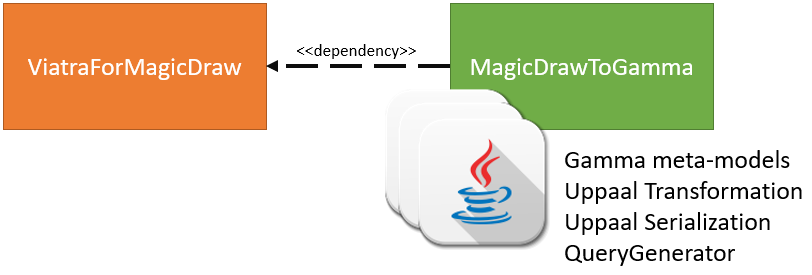
\includegraphics[keepaspectratio, width=120mm]{figures/plan.png}
	\caption{Architektúra koncepció}
	\label{fig:used-gamma}
\end{figure}

\section{Fejlesztőkörnyezet}
 A fejlesztés fejlesztő környezet előkészítésével kezdődött. MagicDraw biztosít egy ún. skeletont Eclipsehez és IntelliJhez is plug-in fejlesztéséhez, de a fejlesztés nem ezek segítségével hanem az IncQueryLabs által készített skeleton felhasználásával valósult meg. Ez már elő volt készítve V4MD használatához.
 
A skeleton egy Eclipse project, viszont Gradlet használ a projekt fordításához és a dependenciák kezeléséhez, ez sokszor inkonzisztenciákhoz vezetett, az egyik legnagyobb probléma a Viatra Querik generálása amit Gradleel nem csak Eclipsel lehet generálni. A kódbázis egy része nem Javában hanem Xtendben íródott, a Viatra trafók implementálása ezzel a nyelvvel egyszerűbb, ahol viszont nem volt indokolt ott Java 8 ban íródott az implementáció.

A dolgozat elkészítése idén a MagicDraw 19-es verziója is elérhető volt a plug-in azonban még nem ehhez, hanem a 18.5-ös verziójához íródott. A kódbázis azonban kompatibilis lehet még az újabb verziókkal is, amennyiben az állapottérképeket érintő meta-modellek nem változnak.

A Gamma dependenciák .jar fájlok formájában vannak a projekthez linkelve. Az eredeti elképzelés szerint, ahol csak lehet a Gamma nem legyen módosítva, viszont egyes részei Viatra 1.6 függőséggel bírtak ami problémákat okozott: a plug-in más verzióját használja az eszköznek, ezért az érintett részekben, az implementáció módosítva lett, hogy azok is Viatra 2-es Api-t használjanak.

A Gamma a verifikációt Uppaal segítségével végzi el, ehhez előállít egy leírást a rendszerről és egy queryt. Utóbbi megírásához biztosít egy QueryGenerátort amivel a felhasználó az Uppaal ismerete nélkül is képes a verifikálandó tulajdonságok definiálására. A QueryGenerator viszont a Gamma Eclipse plug-in részéhez tartozik ezért az implementáció módosítása itt is szükséges volt, hogy önálló részként is képes legyen működni. Ez a funkció teljesen át lett emelve Gammából módosított implementációval a MagicDrawToGammára, jelentős részben azonban az eredeti implementáció dominál.

\subsection{MagicDraw - Gamma transzformáció}

\chapter{Értékelés}
\label{chap:ertekeles}
\section{Alternatíva - kódgenerálás}
A Gamma saját nyelvtanokkal rendelkezik, melyek Xtext segítségével vannak implementálva. Ez a technológia lehetővé teszi, hogy saját szintaxis alapján, lehessen kódot írni és EMF példánymodellt generálni a leírásból.

Ezt a mechanikát ki lehet használni a modell transzformáció alternatívájaként: a MagicDraw modellből \emph{Gamma Statechart Language} szintaxisának megfelelő kódot lehetne generálni és ezt Xtext segítségével leparse-olni.

A visszakövethetőség is megoldható, ehhez a nyelvtant annotációkkal kéne kibővíteni, amik jelölnék az eredeti elemeket.

Ennek előnye, hogy a kimeneteket utána tovább lehetne importálni Eclipse-be és abban folytatni a fejlesztést.

Hátránya viszont, hogy a skálázhatóságot sokkal nehezebb megoldani, és kevésbé flexibilis mint a transzformáció.

\section{Plug-in teljesítménye}

A plug-in teljesítményét leginkább az jellemzi, hogy mennyi idő alatt képes végrehajtani a MagicDraw - Gamma transzformációt. Ennek meghatározására szolgálnak az alábbi mérések. Ezek célja a modell elemek számának és a végrehajtáshoz szükséges idő kapcsolatának vizsgálata.

\subsection{Mérések elvégzéséhez használt specifikációk}

\begin{table}[!h]
	\footnotesize
	\centering
	\begin{tabular}{ l r }
		Processzor & Intel i7-4770 @ 3.40GHz 3,40GHz \\
		Ram memóra & 8Gb\\
		Operációs rendszer & Windows 10 Pro \\
		Java verzió & Java 8 (181) \\
		MagicDraw verzió & 18.5 \\
		MagicDraw maximális heap méret & 2433Mb
	\end{tabular}
	\caption{Méréshez használ specifikációk}
	\label{table:gepspec}
\end{table}

\subsection{Egyszerű állapotgépek triggerrel}

Az egyszerű állapotgépek nem tartalmaznak csak állapotokat állapotátmeneteket és \emph{Signal Event Trigger}eket. A mérések hat különböző mintán lettek futtatva ezeket \aref{table:meres1}. táblázat szemléltei.

\begin{table}[H]
	\footnotesize
	\centering
	\begin{tabular}{ l r r r r r r}
		Név: & m1 & m2 & m3 & m4 & m5 & m6 \\ \hline
		Állapotok száma:  & 10 & 50 & 100 & 500 & 1000 & 2000 \\
		Állapotátmenetek száma: & 10 & 46 & 91 & 461 & 821 & 1641 \\
		\emph{Signal Event Triggerek} száma: & 9 & 45 & 90 & 460 & 820 & 1640
	\end{tabular}
	\caption{Első méréshez használt modellek}
	\label{table:meres1}
\end{table}

A mérések egymás után lettek futtatva ugyan azon a modellen új elemek felvételével az eredményeket \aref{fig:meres1}. ábra szemlélteti. Minden elemet ugyan az a régió tartalmazott és csak egy állapottérkép volt a modellben. Az állapotok és állapotátmenetek tíz hosszú láncokat alkottak. Minden leképzés után a leképzett modell kiírásra került a háttértárra.

\begin{figure}[H]
	\centering
	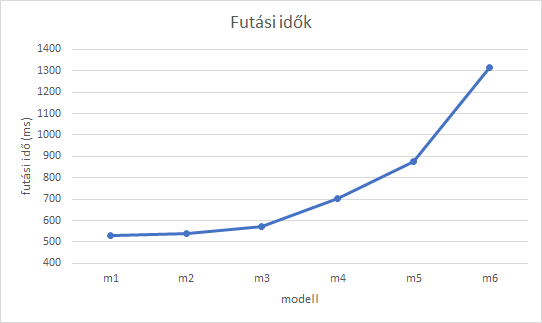
\includegraphics[keepaspectratio, width=140mm]{figures/meres1.png}
	\caption{Első mérés: transzformációk egymás után növekvő modellen}
	\label{fig:meres1}
\end{figure}

A grafikonról leolvasható, hogy az végrehajtási idő közel ugyan olyan arányban nőtt mint ahogy a modell mérete növekedett.

\subsection{Egyszerű állapotgépek őrfeltétellel}

A következő mérések során az állapotátmenetekre őrfeltételek kerülnek. Ezek leképzése Xtext parsert használ. Ennek a méréseknek a célja megvizsgálni az \emph{parse}-olás okozta teljesítmény romlást. Az új modellek és elemszámaikat \aref{table:meres2}. táblázat tartalmazza, az őrfeltétel a következő kifejezés:
\begin{lstlisting}
	true = (true and true) or a > 12
\end{lstlisting}

\paragraph{Megjegyzés:} az őrfeltételben használt \verb+a+ változó deklarálva lett az állapotgépen ennek a leképzése is megvalósul, azonban feltételezhető, hogy ez nem befolyásolja érdemben a mérést.

\begin{table}[H]
	\footnotesize
	\centering
	\begin{tabular}{ l r r r r r r}
		Név: & m1 & m2 & m3 & m4 & m5 & m6 \\ \hline
		Állapotok száma:  & 10 & 50 & 100 & 500 & 1000 & 2000 \\
		Állapotátmenetek száma: & 10 & 46 & 91 & 461 & 821 & 1641 \\
		\emph{Signal Event Triggerek} száma: & 9 & 45 & 90 & 460 & 820 & 1640 \\
		Őrfeltételek száma: & 9 & 45 & 90 & 460 & 820 & 1640
	\end{tabular}
	\caption{Második méréshez használt modellek}
	\label{table:meres2}
\end{table}

\begin{figure}[H]
	\centering
	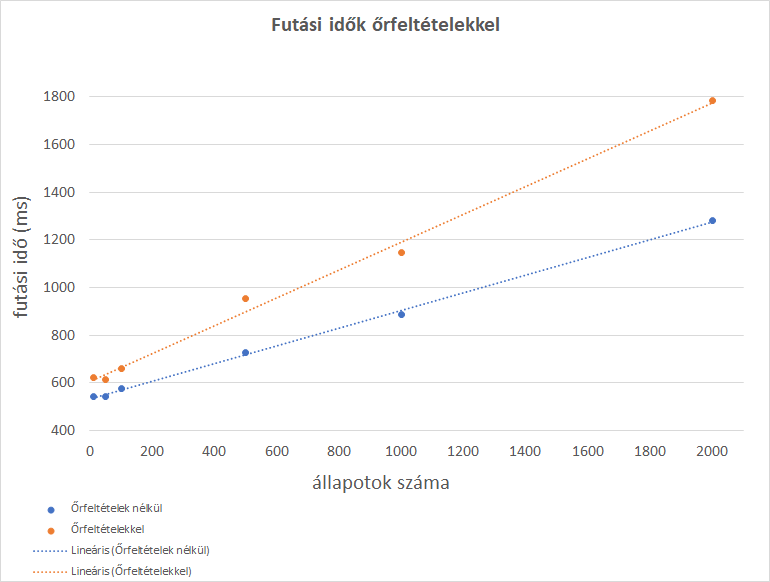
\includegraphics[keepaspectratio, width=140mm]{figures/meres2.png}
	\caption{Második mérés: futási idők őrfeltételekkel}
	\label{fig:meres2}
\end{figure}

Az őrfeltételek alkalmazása minden állapotátmeneten jelentősen megnövelte a futási időt átlag 20-25\%-al, ennek különösen a nagy modellek esetében lehet jelentősége.













\chapter{Összefoglalás}
\label{chap:osszefoglalas}
Dolgozatomban a feladatnak megfelelően bemutattam az állapottérképek formalizmusát és megterveztem egy folyamatot melynek segítségével támogatni lehet ezek formális verifikációját a MagicDraw modellező eszközben. A tervezett eszköz prototípusát megvalósítottam egy plug-in formájában melynek a működését egy esettanulmányon demonstráltam, végül pedig értékeltem az elvégzett munkát és megvizsgáltam a továbbfejlesztési lehetőségeket.

\paragraph{Az elvégzett munka fontosabb kontribúciói:}
\begin{itemize}
	\item Megfeleltetések megtervezése
	\begin{itemize}
		\item Összevetettem a két eszköz Metamodelljét
		\item Kiválasztottam az egymásnak megfeleltethető elemeket
		\item Odafigyeltem a szemantikai különbségekre
	\end{itemize}
	\item Leképzés implementációja
		\begin{itemize}
		\item modell transzformációkra specializált technológiát használtam
		\item az eszközt MagicDraw plug-in formájában valósítottam meg
	\end{itemize}
	\item Fejlesztőkörnyezet kialakítása
		\begin{itemize}
			\item összegyűjtöttem a szükséges dependenciákat
			\item odafigyeltem a tranzitív dependenciák helyes menedzselésére
		\end{itemize}
	\item Lehetővé tettem, hogy a MagicDraw-n belül elvégezhető legyen a verifikáció
			\begin{itemize}
			\item átvettem és módosítottam a Gamma Query Generátor funkcióját
		\end{itemize}

	\item Elméleti megközelítésből értékeltem a munkám
		\begin{itemize}
			\item esettanulmányon mutatom be az elkészült eszközt
			\item áttekintetem az alternatív megvalósítási lehetőségeket
		\end{itemize}	
\end{itemize}
Munkám eredményéül létrejött egy olyan MagicDraw plug-in amivel lehetőség nyílik állapottérképek formális verifikációjának végrehajtásába.

\section{Jövőben elvégzendő munka}

Az eddigi munkám során létrejött eszköz továbbfejleszthető, hogy lehetővé tegye komponens alapú modellek verifikációját is. A jövőben a leképzéseket kiterjesztem, hogy ezeket a modelleket is Gamma modellé lehessen transzformálni és elvégezni a formális verifikációt a rendszeren. Továbbá megtervezek egy olyan új funkciót ami megjeleníti a felhasználóknak azokat az utakat, amik a megszorításaik megsértéséhez vezettek. A felhasználói élmény javítása érdekében validációs szabályokat hozok létre, amik futásidőben figyelmeztetik a felhasználókat azoknak az elemeknek a használatára, amelyek felhasználása nem teszi lehetővé a leképzést, vagy a formális verifikáció végrehajtását. Továbbá megfontolom olyan elemek támogathatóságát, amik az állapottérképek újrahasznosítását teszik lehetővé (\emph{SubmachineState}).


%tervezett
%\include{content/latex-tools}
%\include{content/thesis-format}
%\include{content/template-usage}


% Acknowledgements
%~~~~~~~~~~~~~~~~~~~~~~~~~~~~~~~~~~~~~~~~~~~~~~~~~~~~~~~~~~~~~~~~~~~~~~~~~~~~~~~~~~~~~~
%----------------------------------------------------------------------------
\chapter*{\koszonetnyilvanitas}\addcontentsline{toc}{chapter}{\koszonetnyilvanitas}
%----------------------------------------------------------------------------

Szeretnék köszönetet mondani mindazoknak a feladat elvégzése során segítették a munkám: Farkas Rebekának, aki konzulensemként mindig segítőkész, pozitív hozzáállásával, és szakmai tanácsival, kritikáival segítette a dolgozat létrejöttét. Továbbá Molnár Vincének aki a Gamma Statechart Composition Framework használatát javasolta és ötleteket adott a megvalósítható funkciókra vonatkozóan. Köszönöm továbbá az IncQuery Labs-nak, hogy rendelkezésemre bocsátották a plug-in skeletonjukat, és a náluk töltött szakmai gyakorlatom során szerzett gyakorlati tapasztalatokat, amik jelentősen megkönnyítették az implementáció elkészítését.


% List of Figures, Tables
%~~~~~~~~~~~~~~~~~~~~~~~~~~~~~~~~~~~~~~~~~~~~~~~~~~~~~~~~~~~~~~~~~~~~~~~~~~~~~~~~~~~~~~
%\listoffigures\addcontentsline{toc}{chapter}{\listfigurename}
%\listoftables\addcontentsline{toc}{chapter}{\listtablename}


% Bibliography
%~~~~~~~~~~~~~~~~~~~~~~~~~~~~~~~~~~~~~~~~~~~~~~~~~~~~~~~~~~~~~~~~~~~~~~~~~~~~~~~~~~~~~~
\addcontentsline{toc}{chapter}{\bibname}
\bibliography{bib/mybib}


% Appendix
%~~~~~~~~~~~~~~~~~~~~~~~~~~~~~~~~~~~~~~~~~~~~~~~~~~~~~~~~~~~~~~~~~~~~~~~~~~~~~~~~~~~~~~
%----------------------------------------------------------------------------
\appendix
%----------------------------------------------------------------------------
\chapter*{\fuggelek}\addcontentsline{toc}{chapter}{\fuggelek}
\setcounter{chapter}{\appendixnumber}
%\setcounter{equation}{0} % a fofejezet-szamlalo az angol ABC 6. betuje (F) lesz
\numberwithin{equation}{section}
\numberwithin{figure}{section}
\numberwithin{lstlisting}{section}
%\numberwithin{tabular}{section}

%----------------------------------------------------------------------------
%\section{A TeXstudio felülete}
%----------------------------------------------------------------------------
%\begin{figure}[!ht]
%\centering
%\includegraphics[width=150mm, keepaspectratio]{figures/TeXstudio.png}
%\caption{A TeXstudio \LaTeX-szerkesztő.} 
%\end{figure}


%\label{page:last}
\end{document}
